%  A simple template for Co-author statements in relation to submitting PhD Thesis.
%  2018-09-08 v. 1.0.0
%  Copyright 2018 by Morten Bornø Jensen <mboj@create.aau.dk>
%
%  This is free software: you can redistribute it and/or modify
%  it under the terms of the GNU General Public License as published by
%  the Free Software Foundation, either version 3 of the License, or
%  (at your option) any later version.
%
%  This is distributed in the hope that it will be useful,
%  but WITHOUT ANY WARRANTY; without even the implied warranty of
%  MERCHANTABILITY or FITNESS FOR A PARTICULAR PURPOSE.  See the
%  GNU General Public License for more details.
%
%  You can find the GNU General Public License at <http://www.gnu.org/licenses/>.
%
\documentclass[12pt,oneside]{report}

\usepackage[top=1in, bottom=1.25in, left=1.0in, right=1.0in]{geometry}


%%%%%%%%%%%%%%%%%%%%%%%%%%%%%%%%%%%%%%%%%%%%%%%%
% Language, Encoding and Fonts
% http://en.wikibooks.org/wiki/LaTeX/Internationalization
%%%%%%%%%%%%%%%%%%%%%%%%%%%%%%%%%%%%%%%%%%%%%%%%
% Select encoding of your inputs. Depends on
% your operating system and its default input
% encoding. Typically, you should use
%   Linux  : utf8 (most modern Linux distributions)
%            latin1 
%   Windows: ansinew
%            latin1 (works in most cases)
%   Mac    : applemac
% Notice that you can manually change the input
% encoding of your files by selecting "save as"
% an select the desired input encoding. 
\usepackage[utf8]{inputenc}
\usepackage[danish,english]{babel}
\usepackage{ragged2e}

% Choose the font encoding
\usepackage[T1]{fontenc}


\usepackage{graphicx}
\usepackage{tikz}


% load a colour package
\usepackage{xcolor}
% UniPrint prefers that no colours are used in the template by default.
% However, if you want some colours, then you can easily change the following
%\definecolor{aaublue}{RGB}{0,0,0}% black
\definecolor{aaublue}{RGB}{33,26,82}% dark blue

%%%%%%%%%%%%%%%%%%%%%%%%%%%%%%%%%%%%%%%%%%%%%%%%
% Page Layout and appearance
% http://en.wikibooks.org/wiki/LaTeX/Page_Layout
%%%%%%%%%%%%%%%%%%%%%%%%%%%%%%%%%%%%%%%%%%%%%%%%
%\usepackage[
%  outer=2.0cm, % right margin on an odd page
%  inner=2.0cm, % left margin on an odd page
%  top=2.0cm, % top margin
%  bottom=2.0cm % bottom margin
%  ]{geometry}% Change margins, papersize, etc of the document

\pagestyle{empty} 




\makeatletter
\newcommand{\phdSudent}[1]{\newcommand{\@phdStudent}{#1}}
\newcommand{\thePhdStudent}[0]{\@phdStudent}
\makeatother

% create the paper titlepage
\newcommand{\papertitlepage}[2]{
  {\raggedright \Large \bfseries \color{aaublue}#1 \par} \vskip 1em
  {\raggedright \footnotesize #2 \par}
  \vskip -0.8em
  \noindent\makebox[\linewidth]{\rule{\textwidth}{0.6pt}}
}

\newcommand{\paperInfo}[5]{
  {\justify \small \bfseries Paper Title: \mdseries \itshape #1 \par} \vskip 1em
  {\justify \small \bfseries Paper number in the thesis: \mdseries \itshape #2 \par} \vskip 1em
  {\justify \small \bfseries Publication outlet: \mdseries \itshape #3 \par} \vskip 1em
  {\justify \small \bfseries List of authors: \mdseries \itshape #4 \par} \vskip 1em
  {\justify \small \bfseries PhD Student: \mdseries \itshape \thePhdStudent \par} \vskip 1em
  {\justify \small \bfseries Scientific contribution of the PhD student (all participating PhD students) to the paper: \mdseries \itshape #5 \par} \vskip 1em
}

\newcommand{\authorSignature}[1]{
	{\raggedright \small #1
}	\vskip -0.8em
    \noindent\makebox[\linewidth]{\rule{\textwidth}{0.6pt}}
}

\def\stack{}
\def\stackcount{0}

\def\author#1{{%
#1\ignorespaces
\let\xdo\relax
\count0=\stackcount\relax
\advance\count0 by 1
\xdef\stackcount{\the\count0}%
\toks0{\xdo{#1}}%
\toks2\expandafter{\stack}%
\xdef\stack{\the\toks2 \the\toks0 }}}


\def\printAuthorSignatures{{\count0=0
\def\xdo##1{\advance\count0 by 1
##1 \vskip -0.8em \noindent\makebox[\linewidth]{\rule{\textwidth}{0.6pt}} \vskip 2em }%
\stack}}


\makeatletter
\def\ifshowTemplate{\ifdim\overfullrule>\z@
  \expandafter\@firstoftwo\else\expandafter\@secondoftwo\fi}
\makeatother


\newcommand{\statement}[2]{
	\justify
	\begin{itemize}
	\item[•] \textbf{#1} #2
	\end{itemize}
}


\phdSudent{John Smith}


\begin{document}
\papertitlepage{
	Co-author Statement in Connection with Submission of a PhD Thesis
}{
\justify
	With reference to Ministerial  Order no. 1039 of  August 27 2013 regarding the PhD Degree § 12, article 4, statements from each author about the PhD student’s part in the shared work must be included in case the thesis is based on already published or submitted papers. 
}

\paperInfo{
	% Paper Title
	An Awesome Paper
}{
	% Paper number in the thesis
	A 
}{
	% Publication outlet
	A Brilliant Journal or Conference   
}{
	% List of authors 
	\author{Bruce Wayne},
	\thePhdStudent,
	\author{Charles Francis Xavier},
	\author{Lex Luthor},
	\author{Peter Parker} and
	\author{Clark Kent}
	
}{
	% Scientific contribution of the PhD student (all participating PhD students) to the paper.
 
 \statement{
	PhD Student:
 }{
	 The PhD student contributed to defining the overall problem and proposed the core scientific idea to solve it. The PhD student wrote the entire draft version of the paper, and revised it according to co-authors comments. The PhD student derived the key methodology together with co-author \#1, and the student implemented all simulations. The student identified relevant performance metrics and interpreted the simulation and experimental results with comments from the co-authors.
 }
 \statement{
	Co-author \#1 (also a PhD student):
 }{
	  Co-author \#1 defined the overall problem together with the PhD student. He/she assisted in careful reviewing of the paper and proposed various refinements to the draft proposal made by the student. Further, co-author \#1, together with the other authors, helped interpret the results.
 }
 \statement{
	Co-author \#2 (also a PhD student):
 }{
	  Co-author \#2 (also a PhD student): Co-author \#2 performed the experiments related to the paper, and helped review and improve the paper.
 }
 
 
 
 


}
\vskip 2em
%
%
\raggedright \textbf{Signature, PhD Student}  \vskip 1em

\authorSignature{\thePhdStudent}
%%% Insert your signature. Be sure that it has a transparent background. Comment out if you do not want to include your digital signature.
% You adjust the placement of the signature by adjusting the shift variables in the node setting.
\begin{tikzpicture}[remember picture,overlay]
    \node[xshift=90mm,yshift=8mm]{%
    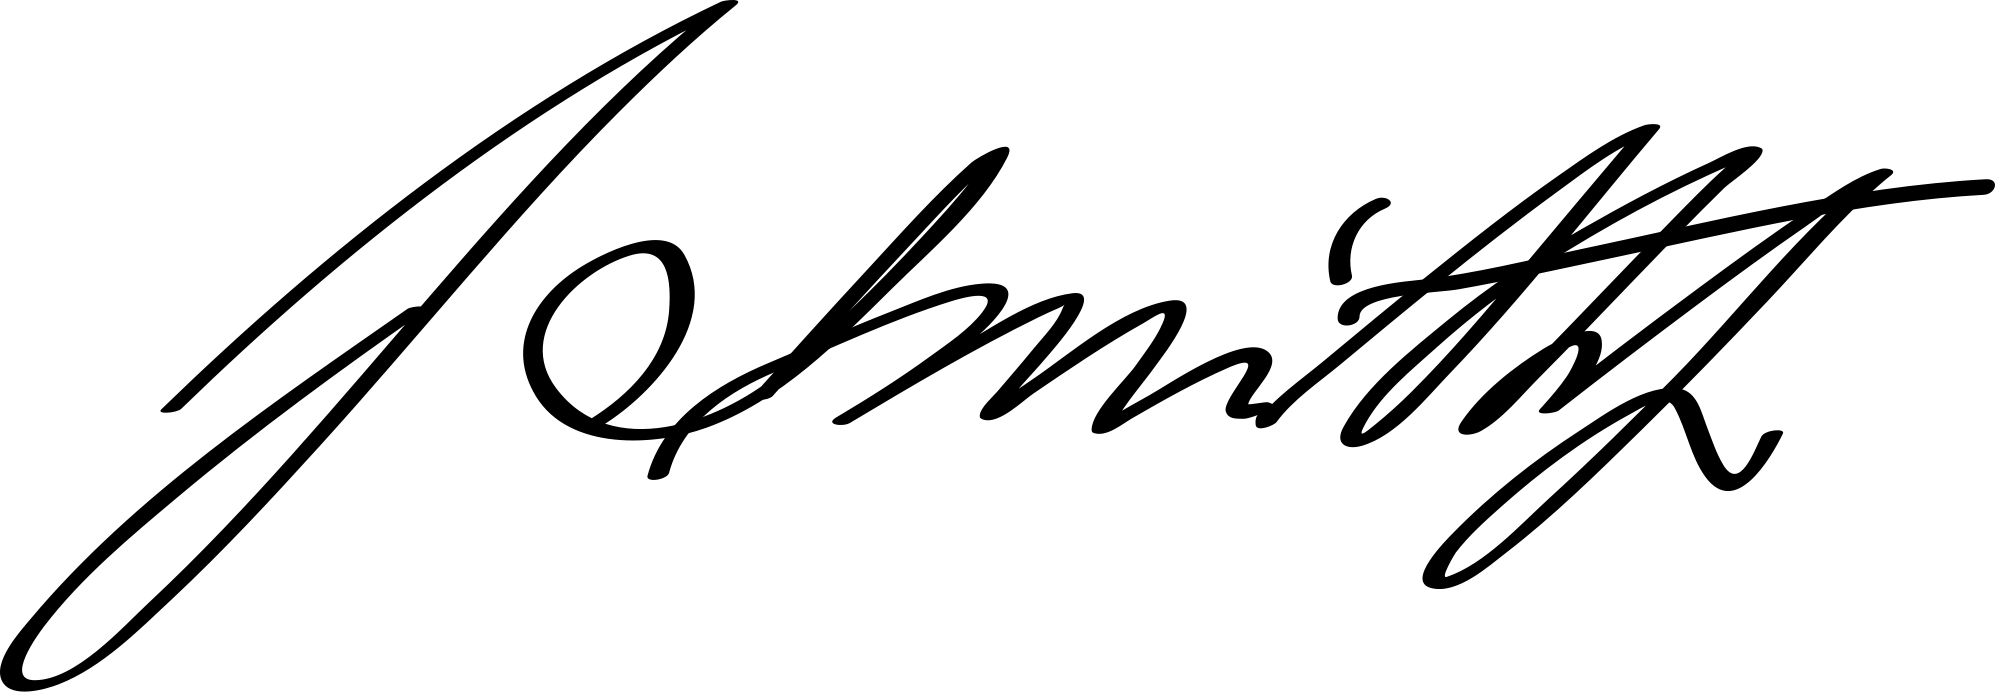
\includegraphics[width=55mm]{signature.png}};
\end{tikzpicture}
%
\vskip 1em
\raggedright \textbf{Signatures, co-authors}  \vskip 1em

\printAuthorSignatures

\end{document}

